% !TeX root = ./PhDThesis.tex

\chapter{Stable trapping of multiple ions}

For a newly built cryogenic trap system, the experimental implementation of stable trapping of multiple ions may take most of the project time before some quantum computing or quantum simulation experiments can be carried out. Experimental implementation of stable trapping of multiple ions involves not only achieving long-lived ion crystals, but also testing a stable standard experimental flow, debugging the experimental platform for various sources of noise, and developing an automatic experimental control system. From a project perspective, it is also a good idea to iterate and optimise the system while achieving stable trapping of multiple ions, and then try to solve the problem when the experiment gets stuck somewhere. Personally, I think more attention should be paid to experimental implementation of stable trapping of multiple ions, because for complex systems, the duplication of effort involved in finding a problem and then solving it can make the total time spent more than the time spent on building a stable experimental system in advance. However, the experimental implementation of stable trapping of multiple ions may not be well defined, and this may become a hole in the methodology.



\section{Semi-automatic experimental control system}

We usually divide the experimental tasks into daily operation tasks and current experiment tasks. The boundary between the two is not clear and we add some daily operation tasks by summarising some of the experimental tasks that have already been solved. Daily operation tasks can also be called experimental setup's parameters calibration tasks. For cryogenic trap systems, daily operation tasks also include the long-term monitoring of some system parameters. In an ideal laboratory environment it is possible to implement an automatic experimental control system, but in most laboratories we can only strive for a semi-automatic experimental control system. This is because some key points have to be controlled and checked by humans, mainly from some uncontrollable human disturbances.

Semi-automatic experimental control system mainly refers to the software system, which contains the front-end system, the back-end system, the database system and the experimental workflow.

\begin{figure}
    \centering
    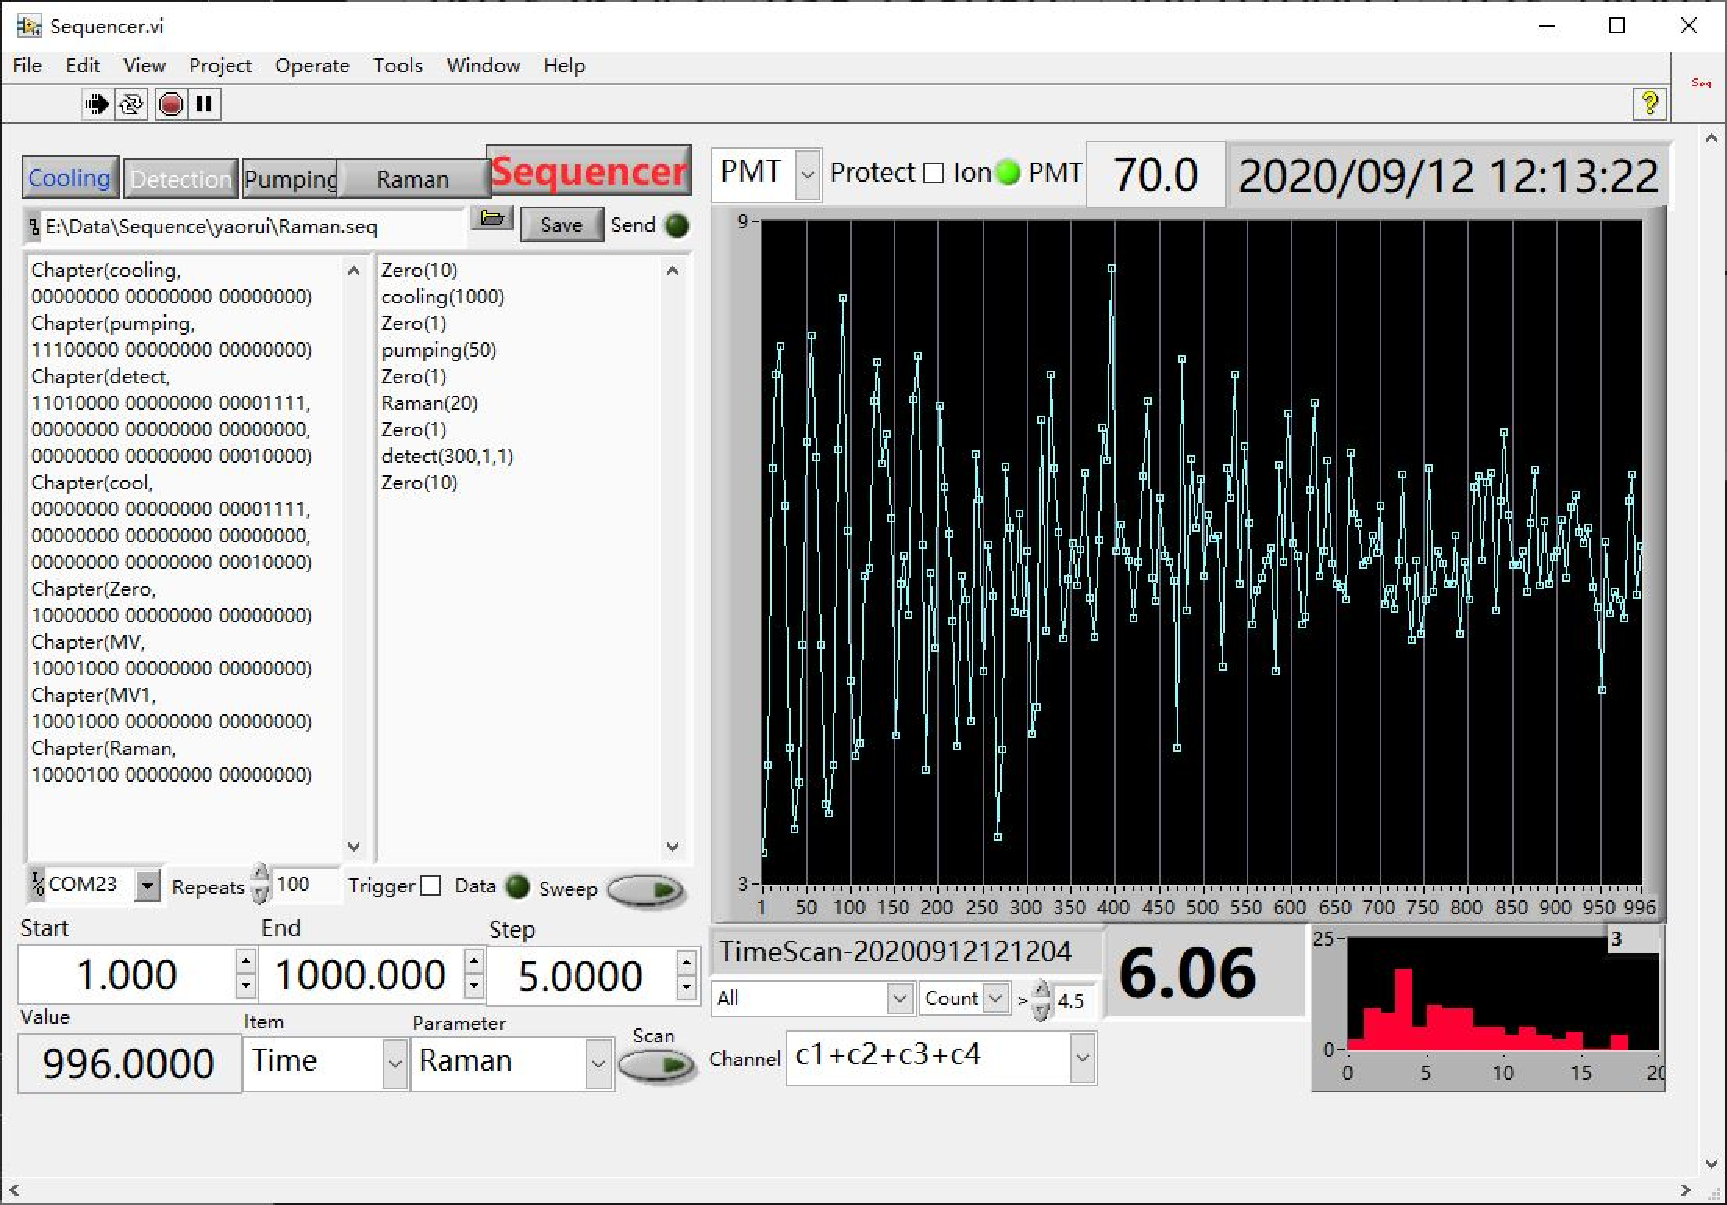
\includegraphics[width=0.8\linewidth]{fig_3_labview_front_end_program.pdf}
    \caption{Labview front-end program (Sequencer).}
\end{figure}

The front-end system is the graphical interface that enables the experimenter to conduct experiments. The popular front-end technologies are client-side front-end technology and Web front-end technology. The more commonly used client-side front-end software in the laboratory are Labview, Mathematica, Matlab and other commercial software, which have rich functions and a friendly programming environment. I have written client-side front-end software based on python and pyqt5, as well as web front-end based on HTML5 technology in the course of my experiments. We can start building the experimental platform without focusing too much on front-end development, as these technologies are not necessary for physics research, and front-end technologies are rapidly growing, so it is possible to leave the front-end system to the professionals.

The back-end system is one of the core elements of the semi-automatic experimental control system. A unified back-end system will speed up the development of the entire semi-automatic experimental control system and facilitate communication and cooperation between project team members. We need the back-end system to control the experimental apparatus in a stable manner and in accordance with the experimental targets. There are a very large number of programming languages for developing back-end systems, suitable for use in the laboratory are C, python, etc. We can also consider using software that integrates front and back ends such as Labview, Mathematica, Matlab, etc. A good back-end system must adhere to lab safety rules, have a good logging system, have a good working state set, be stable over time and have a fast response time. If you are working with multiple people you need to consider version control and documentation for development, such as code hosting. Long-term stability requires a good architecture, as instrument switches and new instrument additions occur frequently and the back-end system should not be offline too often. Instrument control protocols based on sockets and SCPI commands, mqtt protocol based instrument control protocols etc. can be considered. Fast response requires that the back-end program should have a response time of no more than 10-50 ms, which should be met in order to be able to perform complex operations.

\begin{figure}
    \centering
    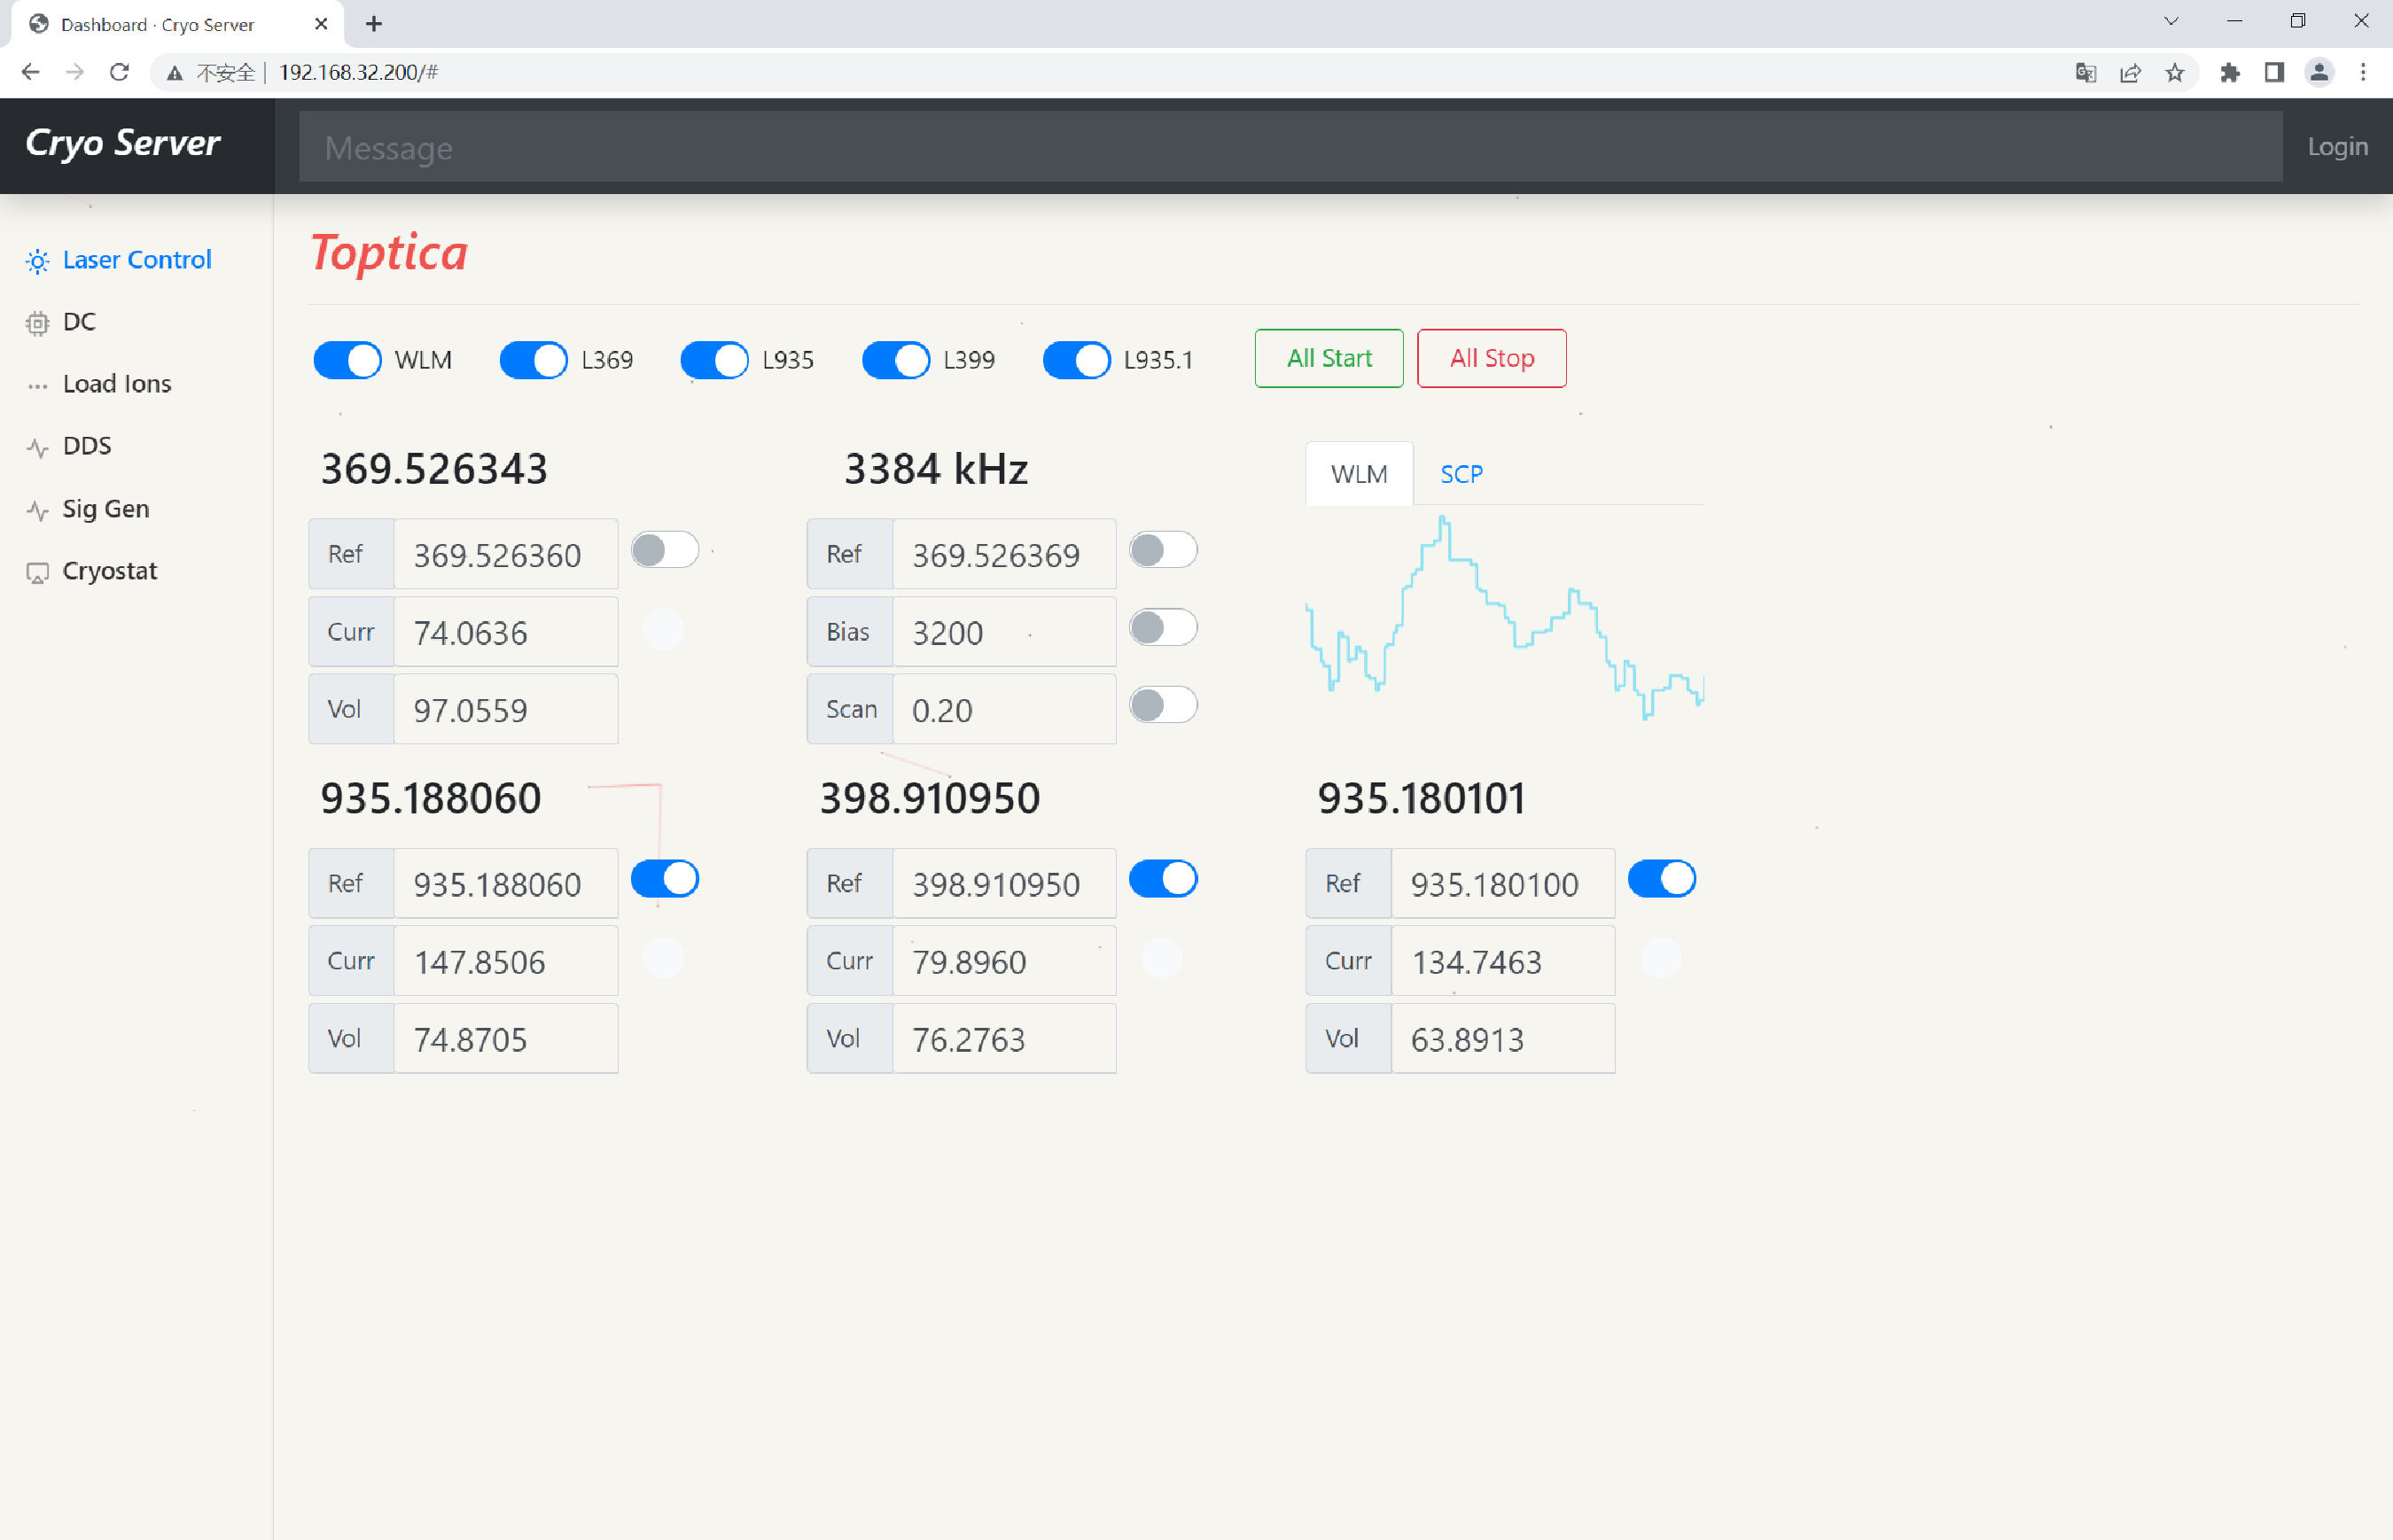
\includegraphics[width=0.8\linewidth]{fig_3_web_front_end_program.pdf}
    \caption{Web front-end program (Lasers etc.).}
\end{figure}

The database system has to take on the task of not only storing data but also taking into account data security. The database system on the experiment should take into account versatility and scalability, and should meet the needs of experimenters of different programming levels to use it. In addition to using SQL databases, InfluxDB, etc., it is also possible to use direct forms of experimental logs and file directory management, or even to use software such as excel directly for recording and management. In short, the database system should be compatible and easy to use as long as it exists and is standardised.

The experimental workflow does not primarily involve work on the code side of things. It is more like a framework bringing together the front-end system, the back-end system and the database system. We need to think about how to easily present the database and access historical data in the front-end system. We need to use it to log, deliver and present the results of experiments. We need to design daily operations and current experiments and easily code the corresponding tasks. Using Mathmatica's notebook or using something like IPython based Jypyter will allow us to do this very well.

During the early build of the lab, we should implement scripted, semi-automated tests under the command of an experimental workflow as soon as possible. With this layout, instead of focusing on front-end system development, we can focus on experimental workflow and database system refinement, while the back-end system can be updated with versioning to patch bugs and improve performance.



\section{Monitor axial electrical potential drift}

We often perform parameter calibration operation at trapping around 10 ions, but if current experimental tasks require ion number between 100 and 200, we need to perform parameter calibration at this ion number scale. This is because repeatedly changing the number of ions in a trap is an operation we do not want to perform. For a well-built blade trap, the upper limit of the ion number of 1D ion chains that can be stably trapped is fixed. When the ion spacing is close to the diffraction limit of the imaging system, we cannot obtain precise information on the ion position from the CCD and the crosstalk between the ions during state detection is too large for high fidelity state detection. In this case we increase the radial trap frequency by increasing the RF power and decrease the axial trap frequency by decreasing the DC voltage. However, there is an upper limit to this method of regulation. When the radial trap frequency is too high, RF heating will occur and the ion crystal will not be stable and will dissolve. In addition, when the ion chain length exceeds the width of the central electrode, we find an asymmetry in the imaging and structure of the ion chain. The asymmetry in the imaging of the ion chain is due to the aberration of the imaging system, we can optimise the imaging system to achieve a field of view of 300 $\mu$m, but it may be more difficult to achieve 600 $\mu$m. The asymmetry of the ion chain structure is due to the asymmetry of the blade electrode and the drift of the background electrical potential.

It is difficult to investigate what the source of the background electrical potential is, but it is objective and there may be more than one source. This phenomenon is clearly observed when we make the ion chain length exceed the width of the central electrode. When the DC voltage is set to a symmetrical value, the ion chain configuration tends to be asymmetrical. This asymmetry also changes over time, either after a day or after a month. It is inevitable that we will do something to the trap in the meantime. This asymmetry can be clearly observed if the oven current is raised to observe the fluorescence of the Yb flux, and the ions can be loaded without turning on the oven during at least one day. This asymmetry changes slowly if more than 200 ions are repeatedly loaded at a time over a period of more than a week, which can be explained by the ions adhering to the surface of the blade after the crystal has been destroyed. We can compensate the background electrical potential with the DC voltage and produce the desired harmonic potential, but when the background electrical potential exceeds the range we can compensate for, we should find a way to eliminate the causes of the background electrical potential drift.

For a complex system, a restart operation is often an effective method. I will try to raise the temperature to room temperature or above 40 K. Over the course of several experiments I have observed that the background electrical potential is removed, which can be quantified by the maximum number of ions that can be stably trapped, or characterised by the asymmetry of the background electrical potential. However, I have occasionally observed that this restart operation does not work completely, and in general this restart operation is effective, but lacks sufficient quantitative data to generalise the factors and values that are truly effective.



\section{Calculate axial electrical potential with 1D ion chains}

We can calculate the axial electrical potential with 1D ion chains. we can use a CCD to measure the position of each ion in the 1D ion chains. this measurement is usually subject to error, and the error is different for different positions of the ions. For a chain of ions, the aberration is smaller for ions near the centre of the field of view and larger for ions near the edge of the field of view. If the ion chain exceeds the edge length of the CCD sensor, we can also measure the position of the ions in sections by moving the objective. In addition to the measurement error, the algorithm used to calculate the ion position can also produce a corresponding error \cite{RN119,RN117,RN228,RN226,RN229,RN227}. Commonly used algorithms for measuring ion positions are linear algorithms based on computer vision, which have the advantage of being fast and able to give results within 10ms. The other algorithm is a fitting-based algorithm, which is less fast and less convergent and is very dependent on the signal-to-noise ratio, but can achieve high accuracy with the right parameters. We can then use the algorithm to find the equilibrium position of the ion chain for a given number of ions and the electrical potential parameter as a calculated value. The difference between the measured and calculated values can then be fed back to the electrical potential as a function of error, so that the parameter with the lowest error, i.e. the axial electrical potential at this point, can be iteratively found.

\begin{figure}
    \centering
    \subcaptionbox{Mathematica code.\label{fig:cal_ion_position_mma_code}}
    {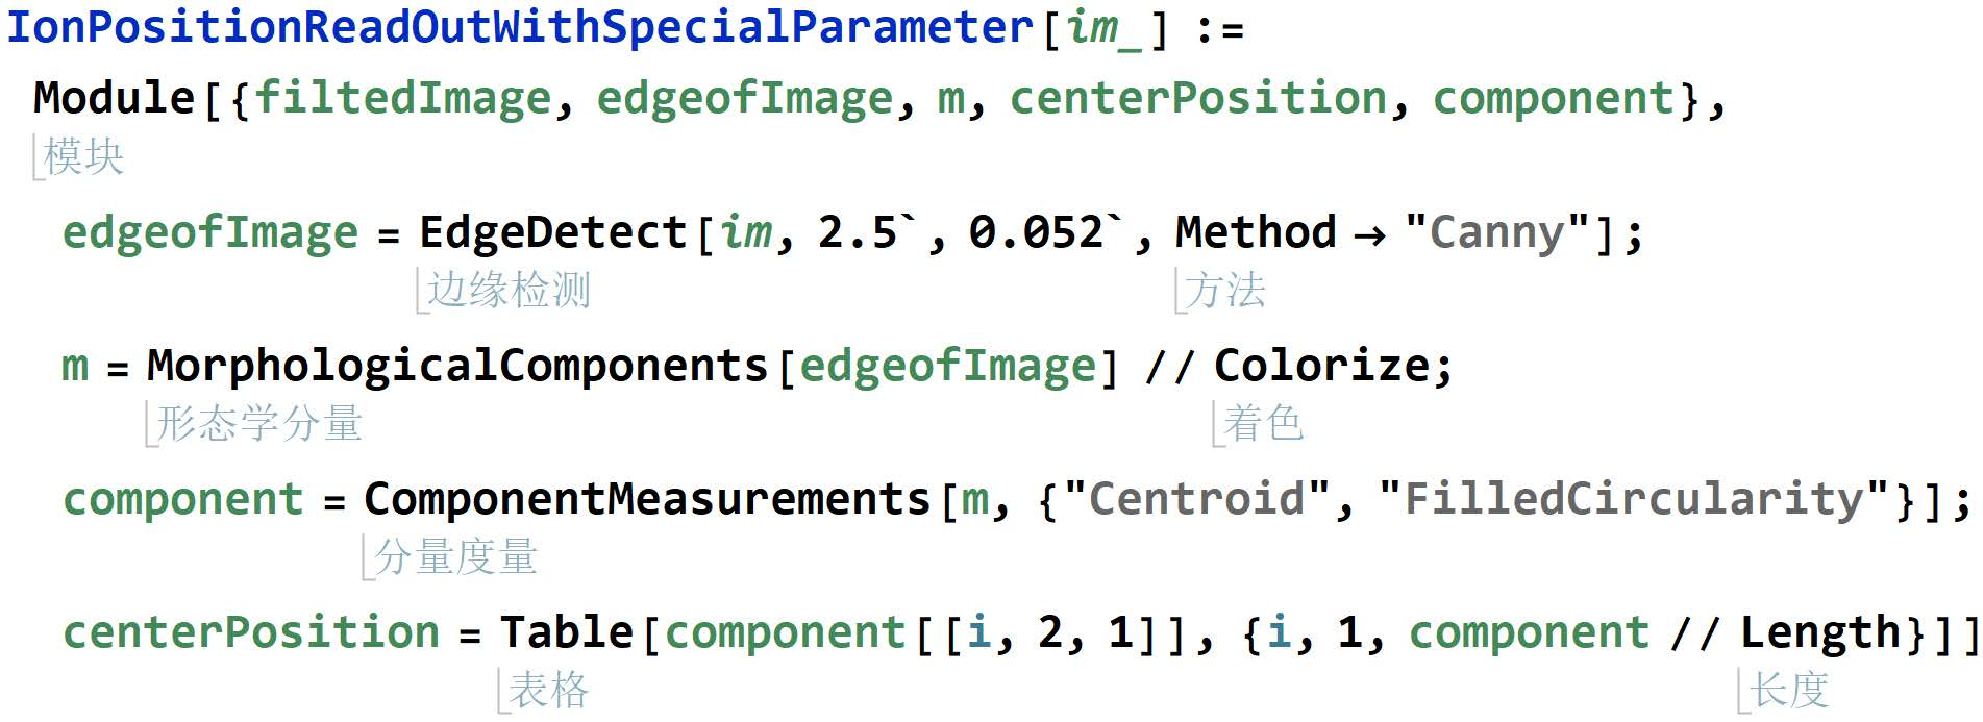
\includegraphics[width=0.8\linewidth]{fig_5_cal_ion_position_mma_code.pdf}}
    \subcaptionbox{Raw image.\label{fig:cal_ion_position_mma_raw}}
    {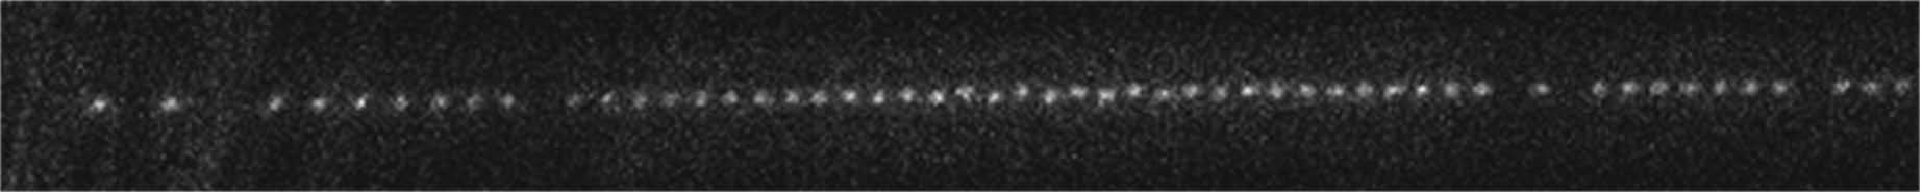
\includegraphics[width=0.4\linewidth]{fig_5_cal_ion_position_mma_raw.pdf}}
    \subcaptionbox{Image after processing.\label{fig:cal_ion_position_mma_result}}
    {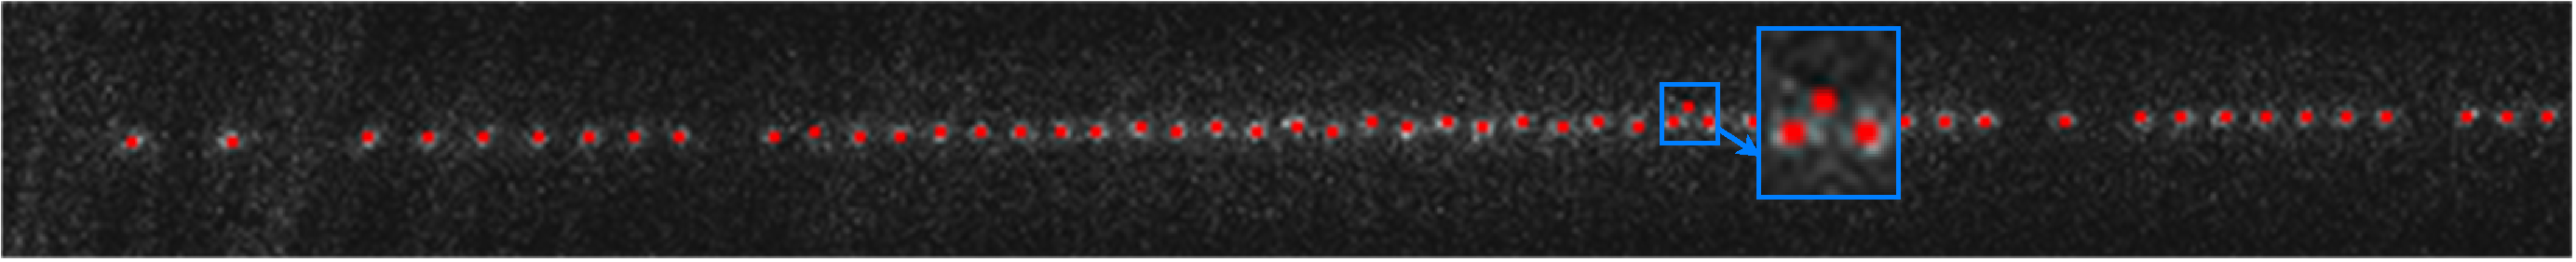
\includegraphics[width=0.4\linewidth]{fig_5_cal_ion_position_mma_result.pdf}}
    \caption{Usage of Mathematica's code to identify a typical ion chain image}
    \label{fig:cal_ion_position_mma}
\end{figure}

Fig~\ref{fig:cal_ion_position_mma_code} shows the use of Mathematica's code to identify a typical ion chain image. Fig~\ref{fig:cal_ion_position_mma_raw} and Fig~\ref{fig:cal_ion_position_mma_result} show the original image and the processed image respectively, with the red dots representing the centre of the identified ions. The background scattered light and the aberration of the image can have an effect on the result of the identification. As can be seen from the recognition results in the blue box in Fig~\ref{fig:cal_ion_position_mma_result}, the trailing of a particular ion may be determined as a new ion, but the conformation of the ion chain precludes this possibility. Optimising the algorithm may be a good idea, but the noise introduced by the imaging system will not be eliminated. Even if the recognition algorithm is optimised using criteria such as no jump in neighbouring ion spacing, ion chain linearity judgement, etc., the noise will still reduce detection fidelity during state detection, and the benefit of reducing noise by optimising the imaging system is much greater. Fig~\ref{fig:cal_ion_position_python} shows code using python to recognise an image of a long ion chain. The algorithms used are similar, so are prone to recognition errors for larger ion chains.

\begin{figure}
    \centering
    \subcaptionbox{Python code.\label{fig:cal_ion_position_python_code}}
    {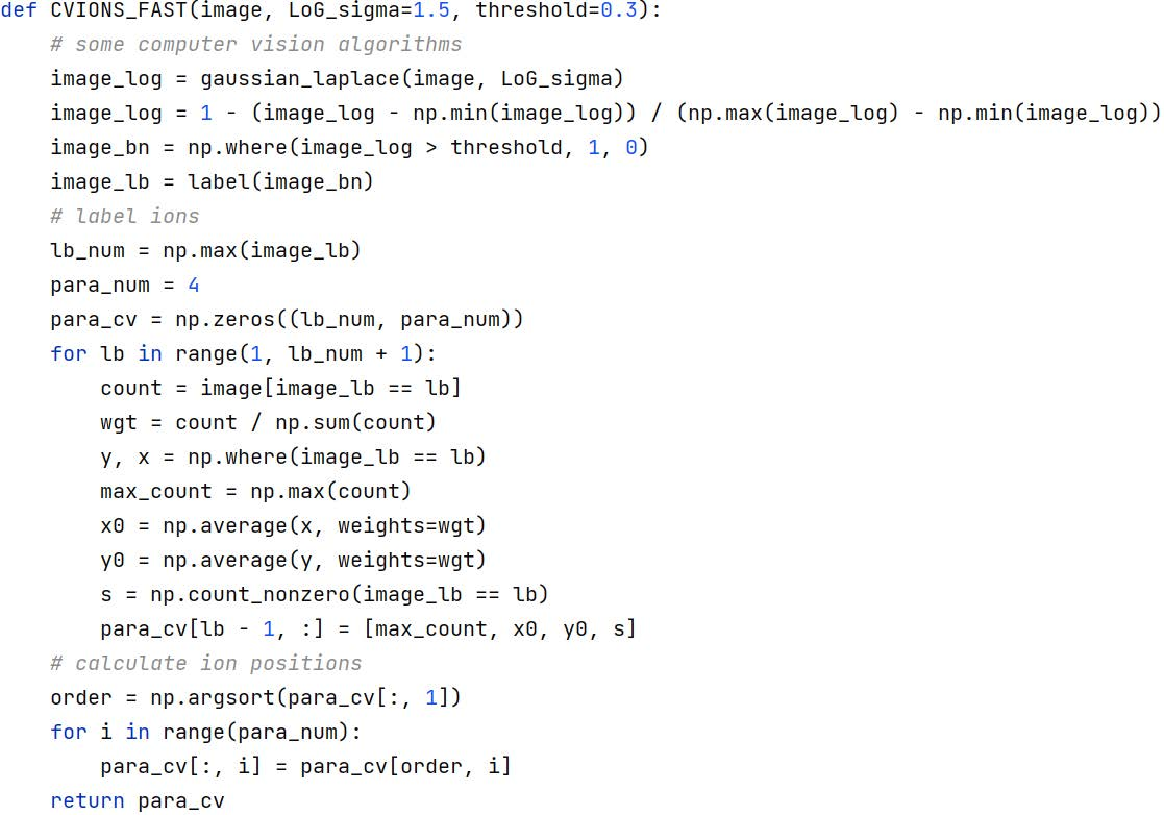
\includegraphics[width=0.8\linewidth]{fig_5_cal_ion_position_python_code.pdf}}
    \subcaptionbox{Image of 245 ions.\label{fig:cal_ion_position_python_raw}}
    {
\includegraphics[width=1.0\linewidth]{fig_5_cal_ion_position_python_245.pdf}}
    \caption{Usage of Python code to calculate 245 ions' position.}
    \label{fig:cal_ion_position_python}
\end{figure}

Now that we are able to obtain information on the location of the ions, we next use a ingenious algorithm proposed by Yukai Wu to calculate the axial electrical potential. The idea of the fitting is very simple. For given trapping potential, we can compute the equilibrium positions of the ions. Then we can adjust the trapping potential to get a best fit of the measured ion positions. For this purpose, it is desired to use a discrete set of parameters to describe the trapping potential. For example, here we use the Legendre polynomials. To get better convergence properties, we scale the axial positions to about $[-1,1]$, which can be recovered in the end.

\begin{figure}
    \centering
    \subcaptionbox{\label{fig:axial_potential_fit_a}}
    {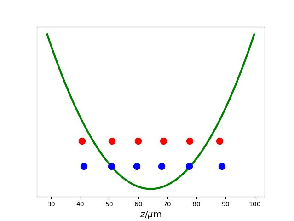
\includegraphics[width=0.4\linewidth]{fig_5_axial_potential_fit_a.pdf}}
    \subcaptionbox{\label{fig:axial_potential_fit_b}}
    {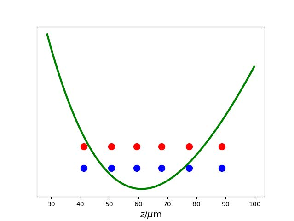
\includegraphics[width=0.4\linewidth]{fig_5_axial_potential_fit_b.pdf}}
    \subcaptionbox{\label{fig:axial_potential_fit_c}}
    {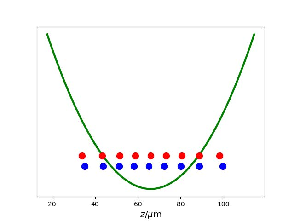
\includegraphics[width=0.4\linewidth]{fig_5_axial_potential_fit_c.pdf}}
    \subcaptionbox{\label{fig:axial_potential_fit_d}}
    {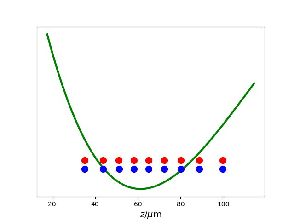
\includegraphics[width=0.4\linewidth]{fig_5_axial_potential_fit_d.pdf}}
    \subcaptionbox{\label{fig:axial_potential_fit_e}}
    {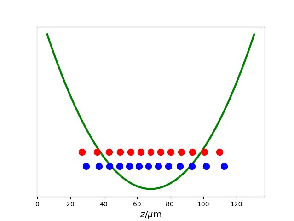
\includegraphics[width=0.4\linewidth]{fig_5_axial_potential_fit_e.pdf}}
    \subcaptionbox{\label{fig:axial_potential_fit_f}}
    {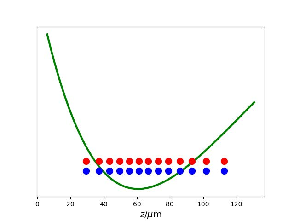
\includegraphics[width=0.4\linewidth]{fig_5_axial_potential_fit_f.pdf}}
    \subcaptionbox{\label{fig:axial_potential_fit_g}}
    {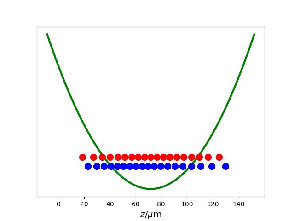
\includegraphics[width=0.4\linewidth]{fig_5_axial_potential_fit_g.pdf}}
    \subcaptionbox{\label{fig:axial_potential_fit_h}}
    {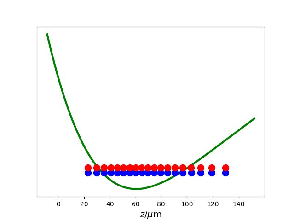
\includegraphics[width=0.4\linewidth]{fig_5_axial_potential_fit_h.pdf}}
    \caption{Fitting results for various ion numbers.}
    \label{fig:axial_potential_fit}
\end{figure}

In Fig~\ref{fig:axial_potential_fit} we present the fitting results for various ion numbers under the same settings of potentials and the CCD camera. Fitting results for (a, b) N = 6, (c, d) N = 9, (e, f) N = 13, (g, h) N = 19. The fitting of the trapping potential uses up to 2nd order polynomials(a, c, e, g) and up to 4th order polynomials (b, d, f, h). The blue and red dots are the measured positions and the fitted ones, respectively. The fitted data are lifted in the vertical direction to better distinguish the two sets of data. The green curves are the fitted axial trap potential. As we can see, 2nd order polynomials do not give good fitting results, but polynomials up to 4th order generally fit well.

\begin{figure}
    \centering
    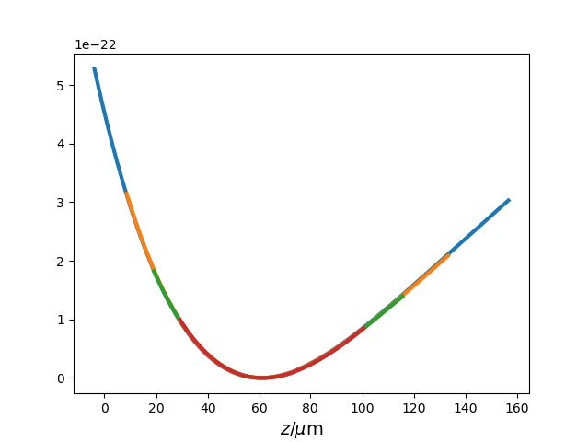
\includegraphics[width=0.4\linewidth]{fig_5_axial_potential_fit_comparison.pdf}
    \caption{Fitted trapping potential for diferrent ion number.}
    \label{fig:axial_potential_fit_comparison}
\end{figure}

Furthermore, we can see in Fig~\ref{fig:axial_potential_fit_comparison} that the fitted potentials for different ion numbers agree well with each other, apart from a constant shift which is not relevant to the equilibrium positions and has been removed. Fitted trapping potential for N = 6 (red), N = 9 (green), N = 13 (orange) and N = 19 (blue) ions.

\begin{figure}
    \centering
    \includegraphics[width=0.4\linewidth]{fig_5_axial_potential_fit_dark_ions.pdf}
    \caption{Fitted trapping potential with dark ions.}
    \label{fig:axial_potential_fit_dark_ions}
\end{figure}

Finally, we comment that the method can be applied to the case where dark ions exist, so long as we can identify the order of the bright and the dark ions. Then we simply use the positions of the bright ones in simulation to fit the trapping potential. As shown in Fig~\ref{fig:axial_potential_fit_dark_ions}, the fitting results is almost the same if the number of dark ions is not too large. The fitting results for the N = 19 case in Fig~\ref{fig:axial_potential_fit} with the ion 6 and ion 9 chosen as dark ions. The fitted potential (green) almost overlaps with the previous one (black) where
all the ions are bright.



\section{Fitting the electrical potential coefficient for each electrode}

For a fixed electrical potential, we can capture different numbers of ions, as shown in Fig~\ref{fig:fit_electrical_potential_coefficient}, 2, 12, 24, 34, 42. For each image, we can calculate the position of the ion and fit it to the electrical potential at that time. Red circles and dots on the right-hand side indicate the calculated position of the ion and the equilibrium position of the ion at the fitted electrical potential, respectively. The black dots indicate the presence of dark ions. The electrical potential can be expressed as

\begin{equation}
    \phi_n(x)=\sum_{i=1}^n \alpha_i P_i(x), x=z / l_0,
\end{equation}

where $z$ is the true position of the ion, $l_0$ is half the length of the ion chain, $P_i(x)$ is the Legendre polynomial of degree i and $\alpha_i$ is the coefficient of the expansion.

Since the electrical potential has not changed, the fit should be consistent for different numbers of ions. As shown in Table~\ref{tab:fitting_the_electrical_potential_coefficient}, the coefficients of the Legendre polynomial have consistent convergence for data with 2 to 42 ions.

\begin{figure}
    \centering
    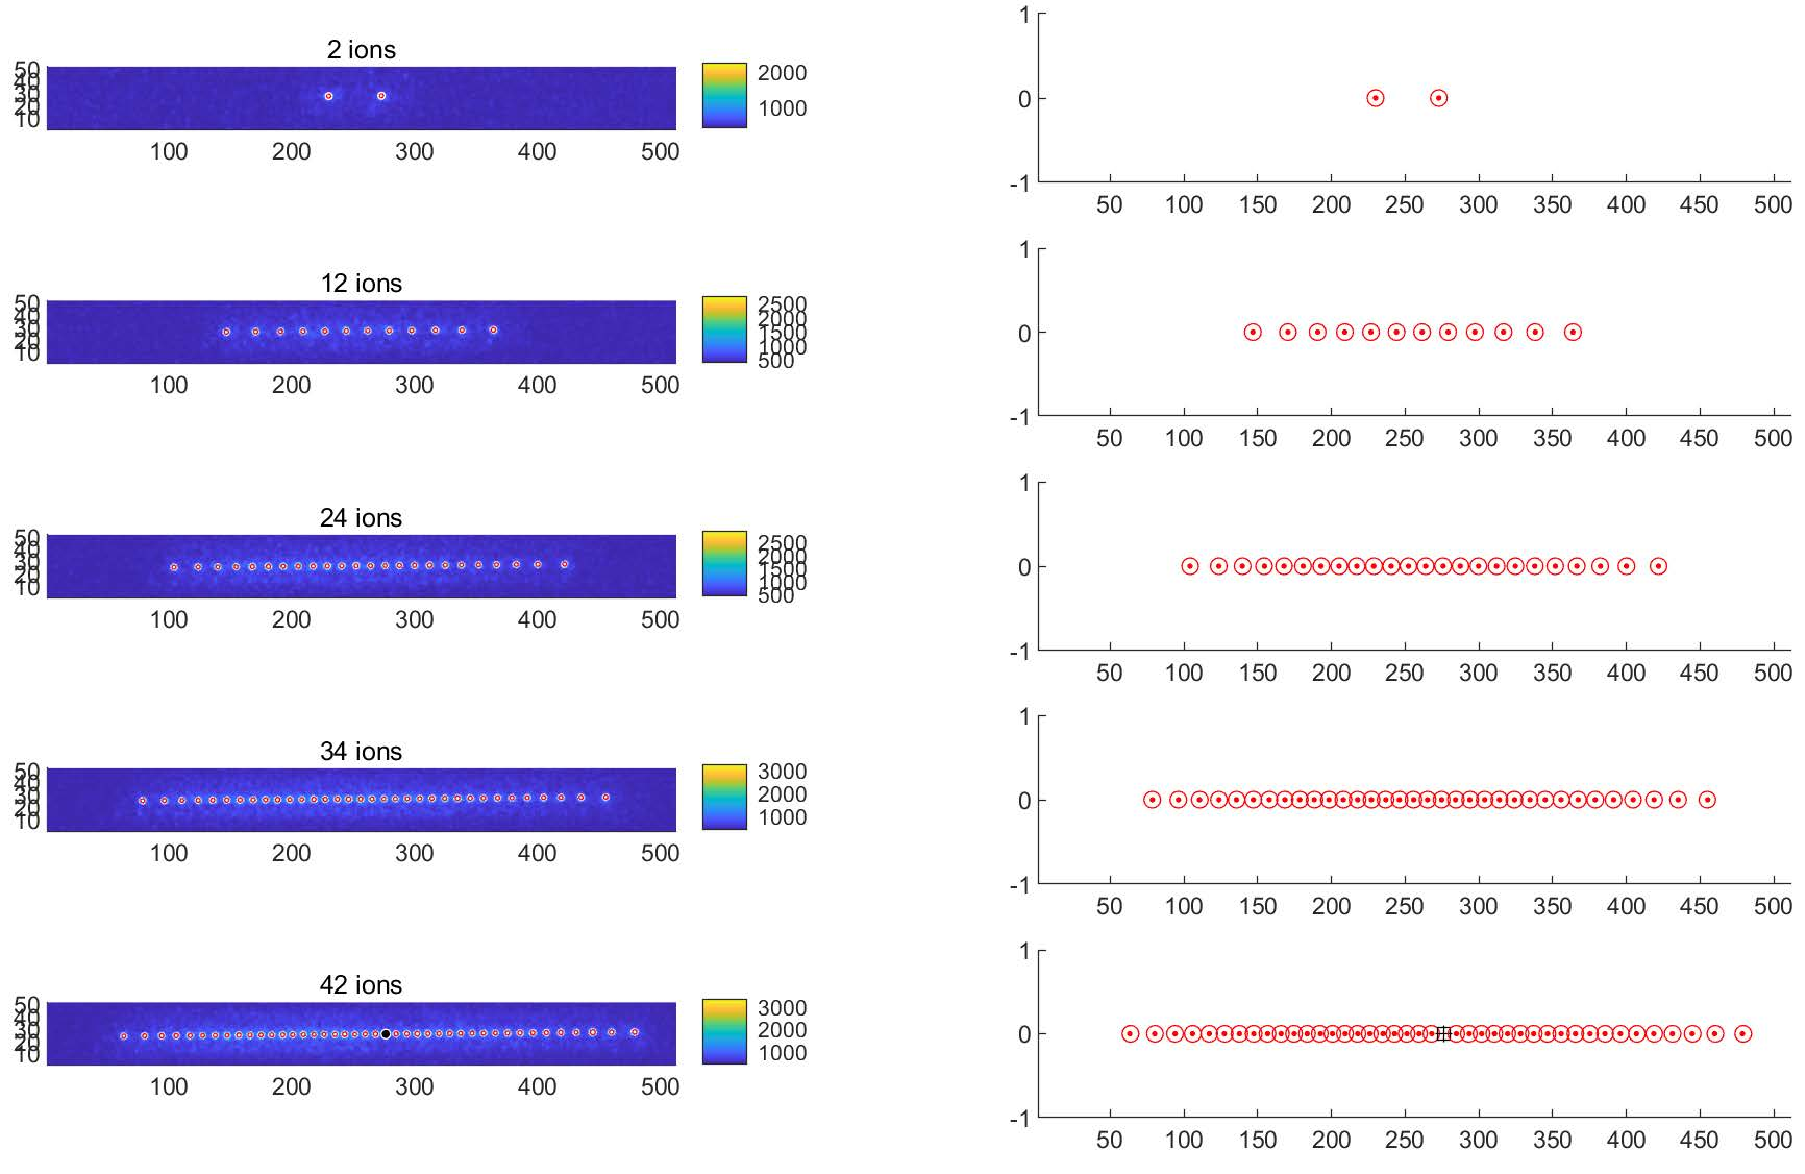
\includegraphics[width=0.8\linewidth]{fig_5_fit_electrical_potential_coefficient.pdf}
    \caption{Fit trapping potential up to 42 ions.}
    \label{fig:fit_electrical_potential_coefficient}
\end{figure}

\begin{table}
    \centering
    \caption{Fitting the electrical potential coefficient}
    \begin{tabular}{lllll}
        \toprule
        Ion number & $\alpha_1$ & $\alpha_2$ & $\alpha_3$ & $\alpha_4$ \\
        \midrule
        2          & 7.59183    & 212.463    & 0          & 0          \\
        12         & 12.5574    & 207.098    & -45.04     & 40.0967    \\
        24         & 10.8866    & 204.913    & -50.165    & 48.4474    \\
        34         & 10.8904    & 204.944    & -49.784    & 48.0492    \\
        42         & 10.7205    & 205.988    & -55.486    & 47.6406    \\
        \bottomrule
    \end{tabular}
    \label{tab:fitting_the_electrical_potential_coefficient}
\end{table}

If we were to use this algorithm directly to calculate the coefficients of the electrical potential at different voltages, we would end up with scattered results due to overfitting. So we need to assume that the coefficient of the electrical potential is fixed for each electrode and then decompose the electrical potential from the actual voltage into the sum of each electrode,

\begin{equation}
    \alpha_i=\sum_{s=1}^5 \alpha_i^s U_s
\end{equation}

where $\alpha_i^s$ the coefficient of the electrical potential generated by each pair of DC electrodes, $s$ is the order number of the electrodes, there are 5 pairs of electrodes in total. And $U_s$ is the voltage applied to the electrodes.

\begin{figure}
    \centering
    \subcaptionbox{\label{fig:fit_the_electrical_potential_coefficient_for_each_electrode_image}}
    {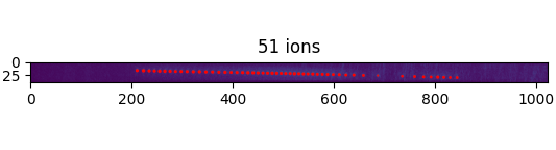
\includegraphics[width=0.8\linewidth]{fig_5_fit_the_electrical_potential_coefficient_for_each_electrode_image.pdf}}
    \subcaptionbox{\label{fig:fit_the_electrical_potential_coefficient_for_each_electrode_1}}
    {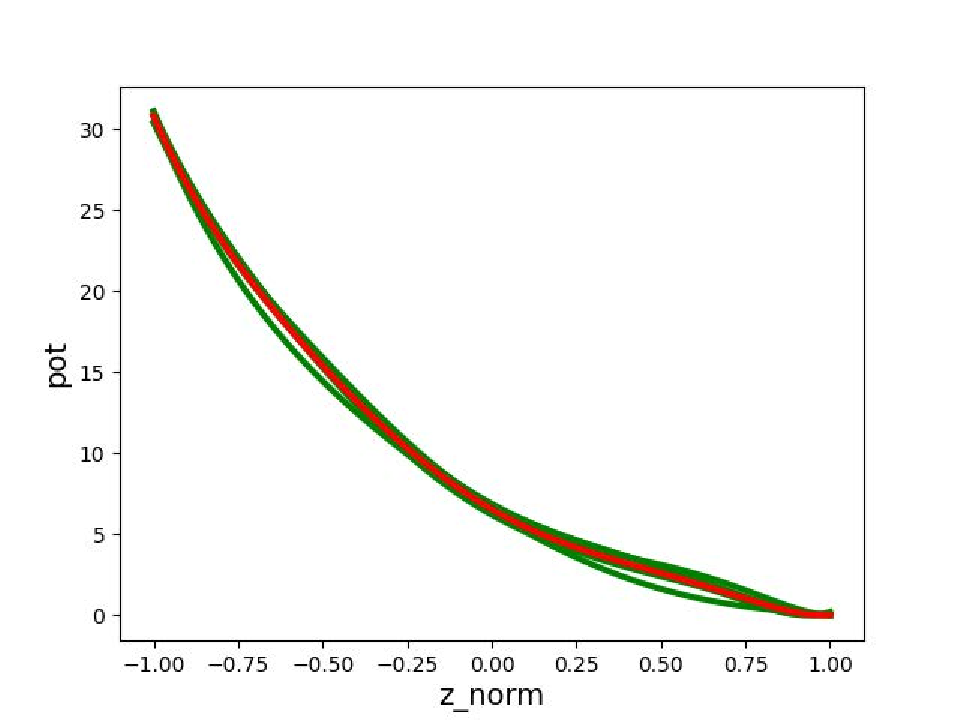
\includegraphics[width=0.3\linewidth]{fig_5_fit_the_electrical_potential_coefficient_for_each_electrode_1.pdf}}
    \subcaptionbox{\label{fig:fit_the_electrical_potential_coefficient_for_each_electrode_2}}
    {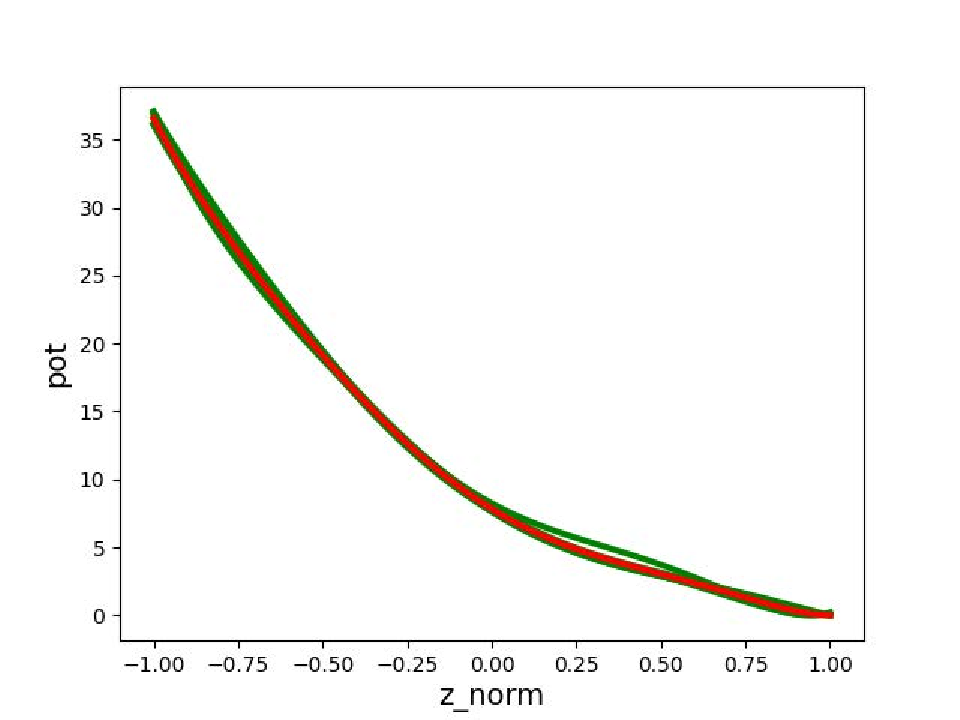
\includegraphics[width=0.3\linewidth]{fig_5_fit_the_electrical_potential_coefficient_for_each_electrode_2.pdf}}
    \subcaptionbox{\label{fig:fit_the_electrical_potential_coefficient_for_each_electrode_3}}
    {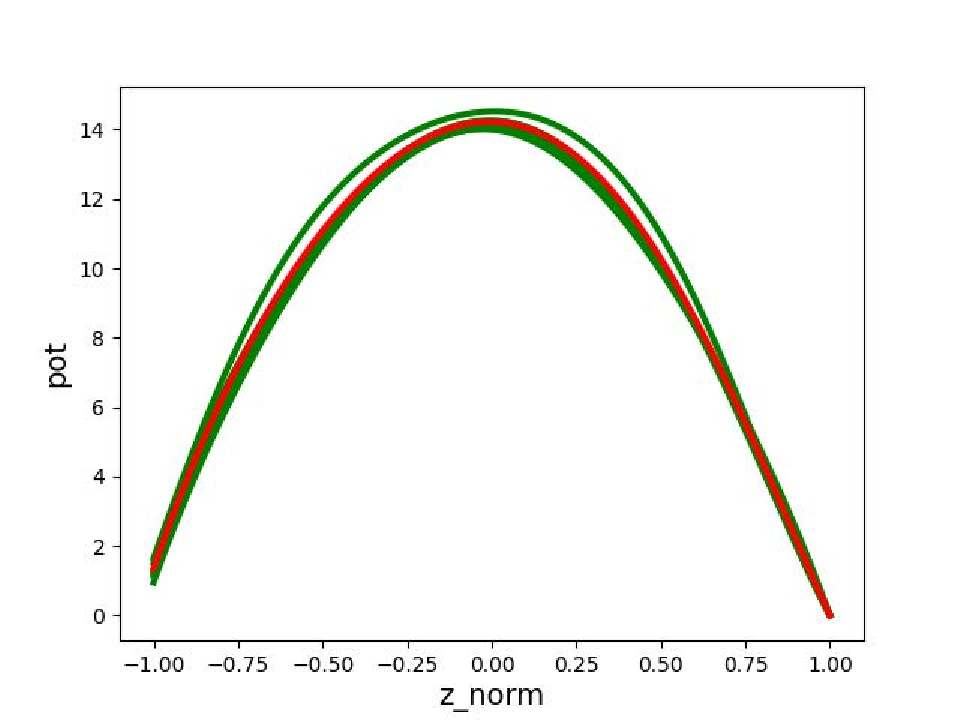
\includegraphics[width=0.3\linewidth]{fig_5_fit_the_electrical_potential_coefficient_for_each_electrode_3.pdf}}
    \subcaptionbox{\label{fig:fit_the_electrical_potential_coefficient_for_each_electrode_4}}
    {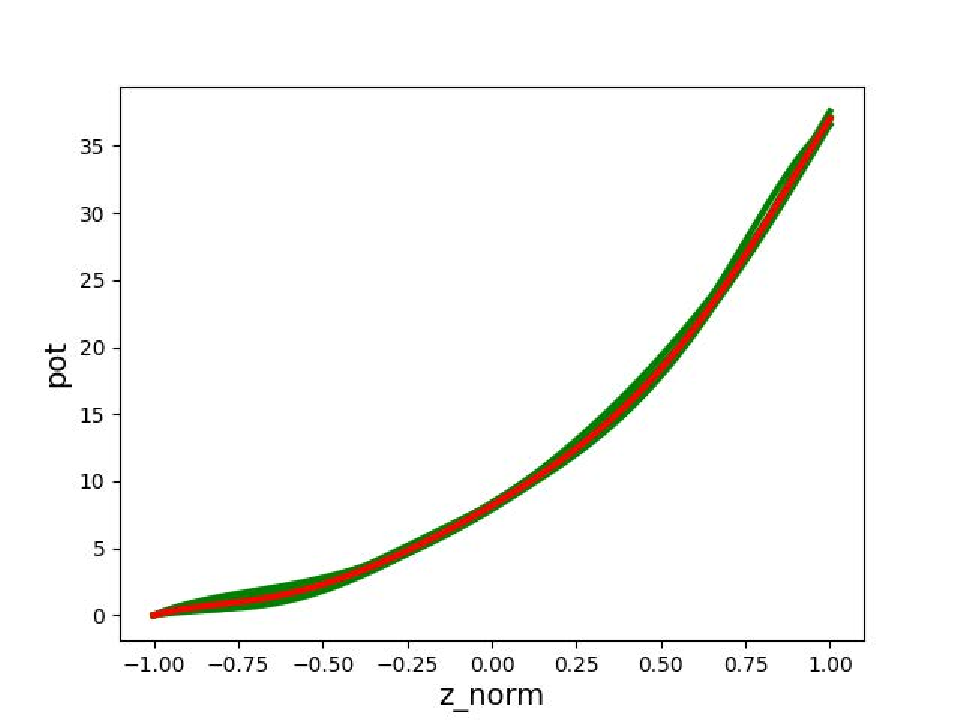
\includegraphics[width=0.3\linewidth]{fig_5_fit_the_electrical_potential_coefficient_for_each_electrode_4.pdf}}
    \subcaptionbox{\label{fig:fit_the_electrical_potential_coefficient_for_each_electrode_5}}
    {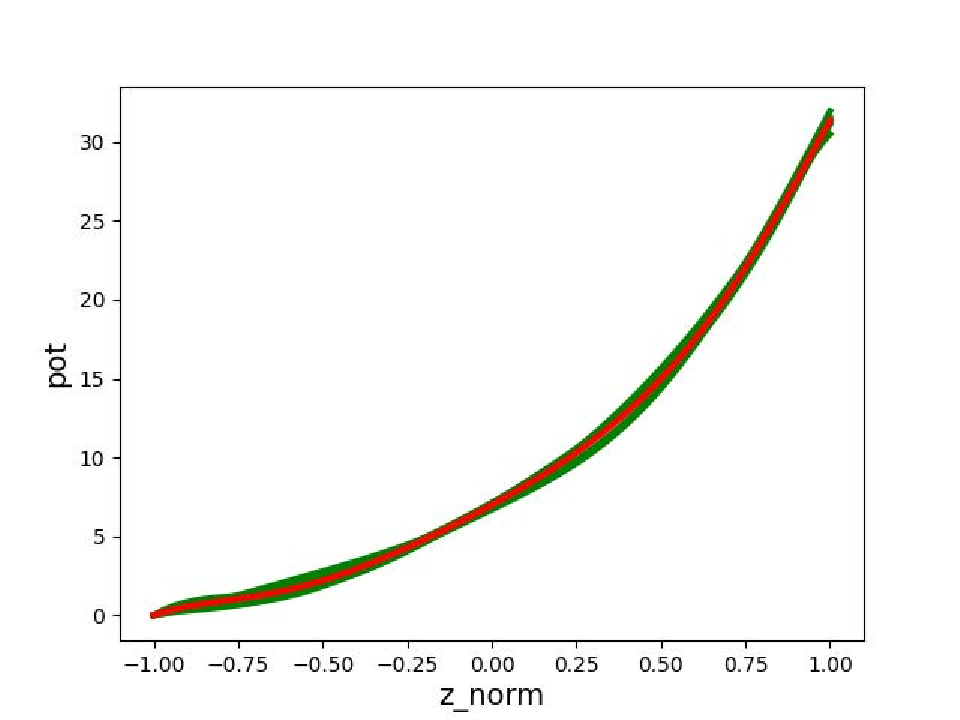
\includegraphics[width=0.3\linewidth]{fig_5_fit_the_electrical_potential_coefficient_for_each_electrode_5.pdf}}
    \subcaptionbox{\label{fig:fit_the_electrical_potential_coefficient_for_each_electrode_image_2}}
    {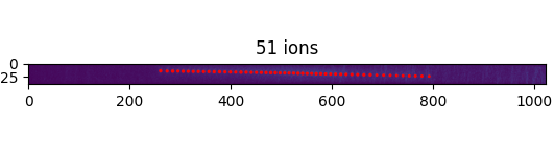
\includegraphics[width=0.8\linewidth]{fig_5_fit_the_electrical_potential_coefficient_for_each_electrode_image_2.pdf}}
    \caption{Fit the electrical potential coefficient for each electrode.}
    \label{fig:fit_the_electrical_potential_coefficient_for_each_electrode}
\end{figure}

I trapped 51 ions at a fixed electrical potential, as shown in Fig~\ref{fig:fit_the_electrical_potential_coefficient_for_each_electrode_image}. Although the applied electrode voltage is symmetrical, the resulting potential field is asymmetrical, which is not what we want. I then added a fixed voltage to each pair of electrodes, at which point I could find the new electrical potential. The single result may have a large error, but if the voltage is increased in equal steps, it can be fitted to give $\alpha_i^s$. In Fig~\ref{fig:fit_the_electrical_potential_coefficient_for_each_electrode}(b)-(f), I have plotted the electrical potential generated by the 5 pairs of electrodes. The green line represents the increase in electrical potential for equal steps of increasing voltage, and you can see that the increase in electrical potential is fixed. The red line represents the average of these data, and I think this value can represent the coefficient of electrical potential generated by each pair of DC electrodes. Next I calculated at what voltage settings this asymmetry could be compensated for and then achieved the result shown in Fig~\ref{fig:fit_the_electrical_potential_coefficient_for_each_electrode_image_2}, where the ions are equally spaced.



\section{Stabilization of axial electrical potential}

When the number of ions becomes larger, we encounter some challenges. On the one hand the applicability of the algorithm can be problematic. For a quasi-1D chain of 126 ions as shown in Fig~\ref{fig:stabilization_of_axial_electrical_potential_image}, the original algorithm fails due to the emergence of the zig-zag configuration. Since the original algorithm is only valid for 1D ion chains, we can consider optimisation algorithms to solve this problem. On the other hand, when experimental parameters such as image aberrations, adjustable range of voltages, etc. can gradually become a major source of noise, they can cause excessive errors or be too unstable, and we can solve this problem by refining the physical system.

\begin{figure}
    \centering
    \subcaptionbox{\label{fig:stabilization_of_axial_electrical_potential_image}}
    {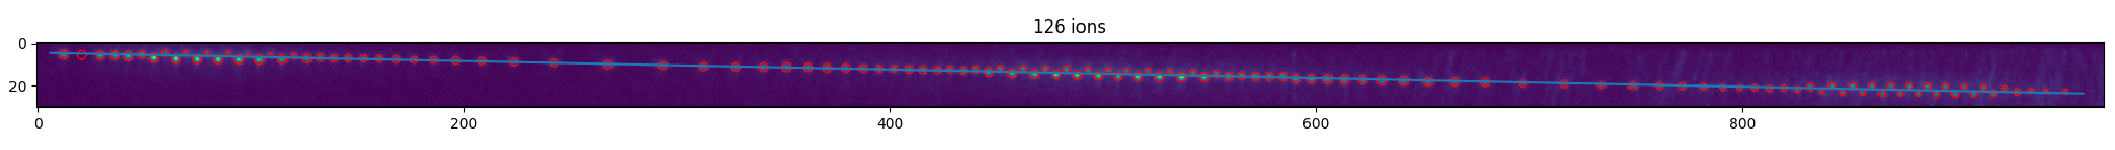
\includegraphics[width=0.8\linewidth]{fig_5_stabilization_of_axial_electrical_potential_image.pdf}}
    \subcaptionbox{\label{fig:stabilization_of_axial_electrical_potential_1}}
    {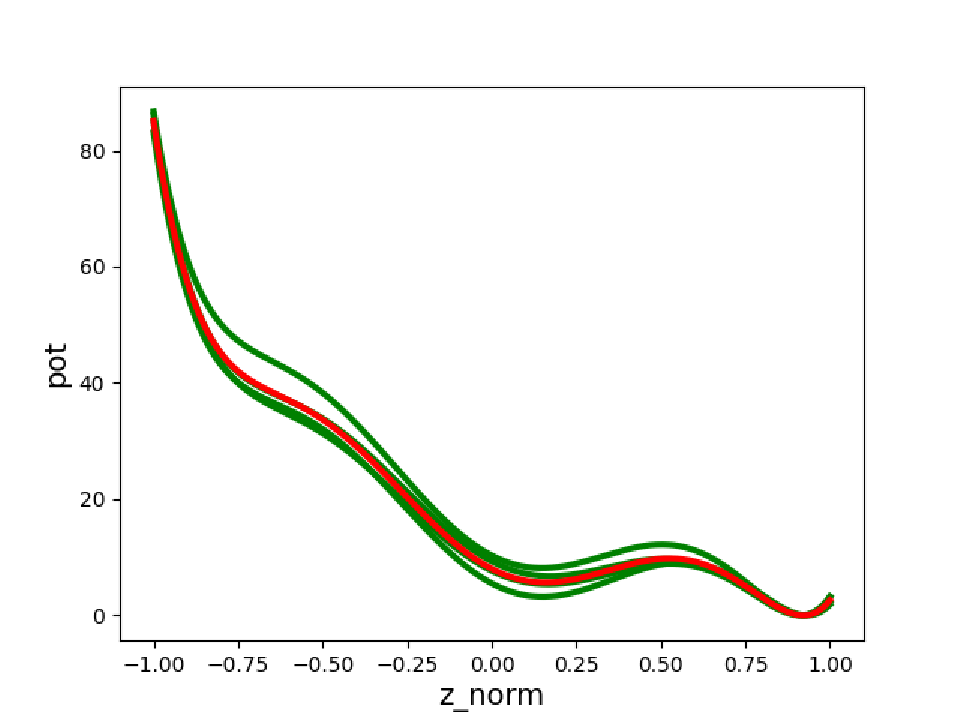
\includegraphics[width=0.3\linewidth]{fig_5_stabilization_of_axial_electrical_potential_1.pdf}}
    \subcaptionbox{\label{fig:stabilization_of_axial_electrical_potential_2}}
    {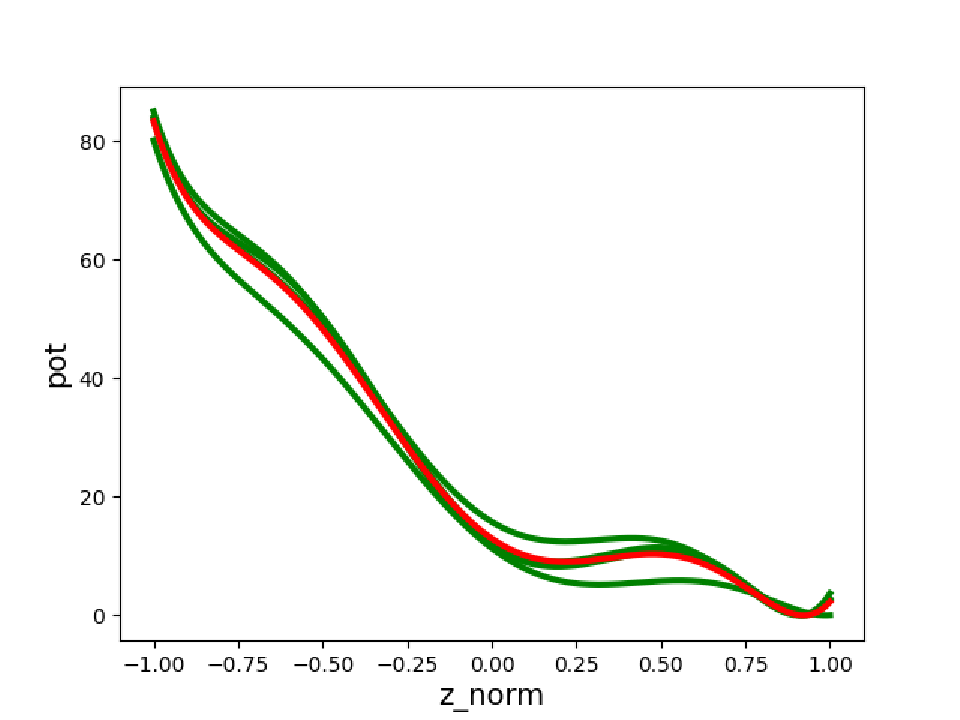
\includegraphics[width=0.3\linewidth]{fig_5_stabilization_of_axial_electrical_potential_2.pdf}}
    \subcaptionbox{\label{fig:stabilization_of_axial_electrical_potential_3}}
    {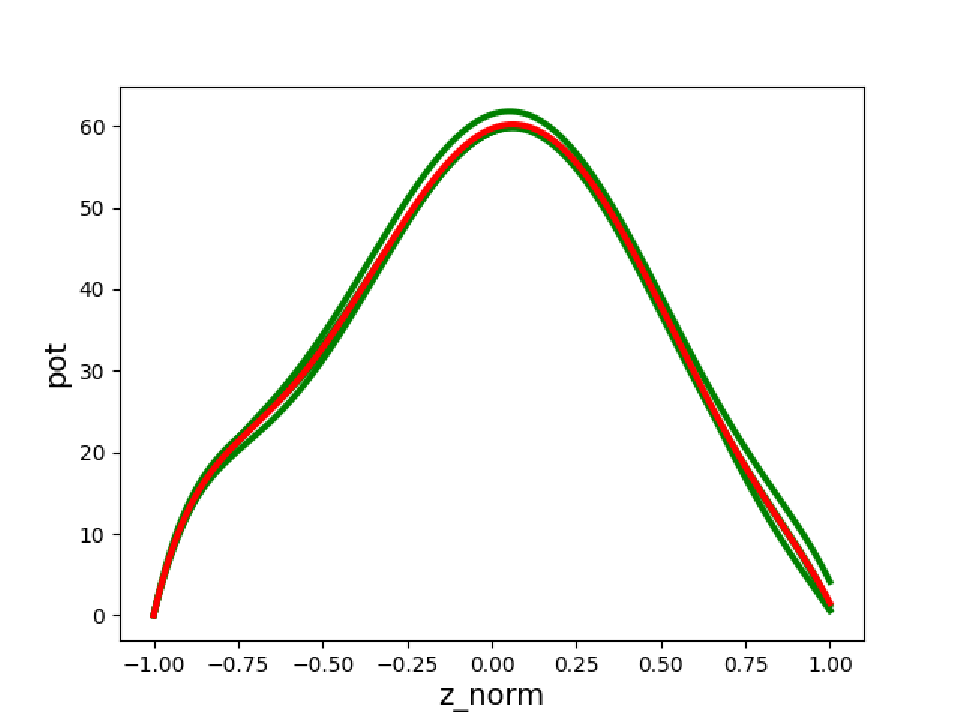
\includegraphics[width=0.3\linewidth]{fig_5_stabilization_of_axial_electrical_potential_3.pdf}}
    \subcaptionbox{\label{fig:stabilization_of_axial_electrical_potential_4}}
    {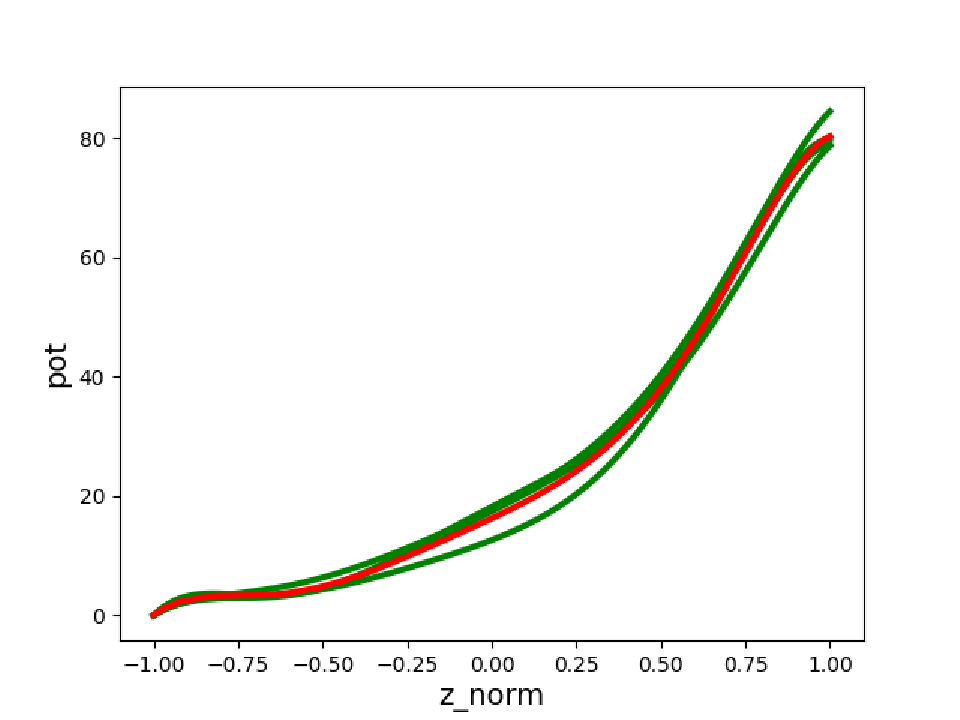
\includegraphics[width=0.3\linewidth]{fig_5_stabilization_of_axial_electrical_potential_4.pdf}}
    \subcaptionbox{\label{fig:stabilization_of_axial_electrical_potential_5}}
    {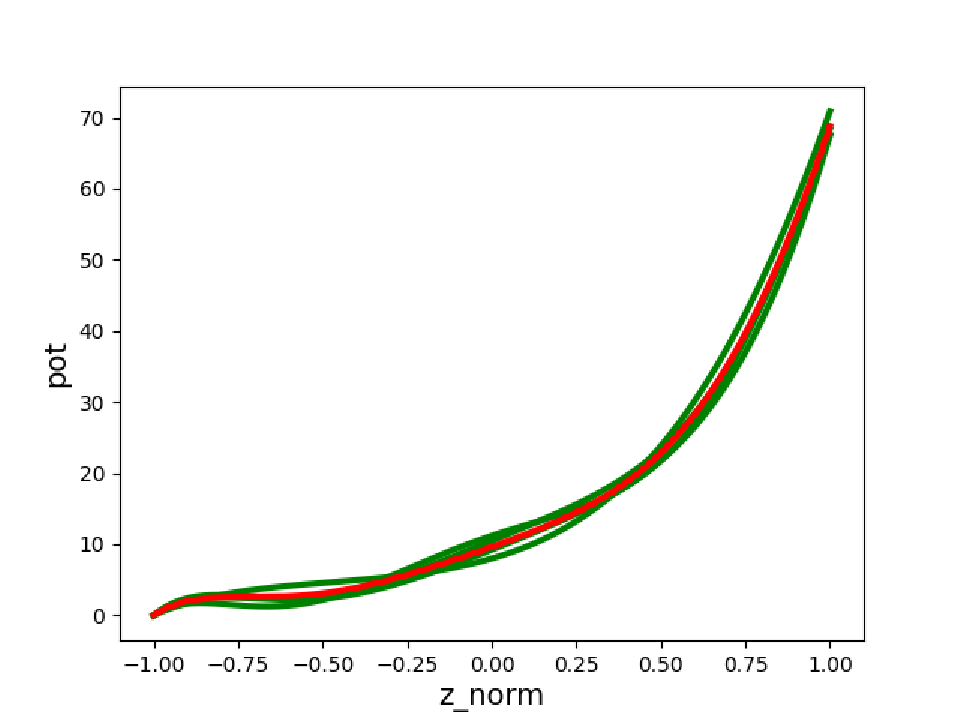
\includegraphics[width=0.3\linewidth]{fig_5_stabilization_of_axial_electrical_potential_5.pdf}}
    \caption{Fit the electrical potential coefficient with a 126-ions quasi-1D chain.}
    \label{fig:stabilization_of_axial_electrical_potential}
\end{figure}

There are a number of ideas for optimisation algorithms, one simple idea is to abandon the calculation of the theoretical equilibrium position for a given electrical potential and take the equilibrium position of the ion directly from the image and invert the electrical potential at this point according to Coulomb's law. Using this method we can obtain the electrical potential for five pairs of electrodes as shown in Fig~\ref{fig:stabilization_of_axial_electrical_potential}(b)-(f). It can be seen that at this scale of ion numbers the error becomes larger.